
\subsection{Product spherical model and Hermite coordinates}
\label{subsec:product-spherical-model}

\paragraph{Role of this subsection.}
This subsection fixes the product-measure model and the coordinate system used in the geometry argument below. We restrict the dynamics to a product ansatz
\(\mu_t=\mu_{1,t}\otimes\mu_{2,t}\). Thus the flow considered here is the product Wasserstein gradient flow on the two marginals, rather than the unrestricted WGF on all couplings. This convention is natural for two interacting mean-field networks and keeps each marginal on the sphere.

\subsubsection{Product-measure objective and product WGF}

We first define the product state space, the fitting loss, and the metric
regularizer used in the curvature example.

We consider a product mean-field neural network whose two marginals live on the sphere. The fitting term compares the matrix-valued product of two mean-field neural networks, while a metric regularizer softly anchors each marginal to an antipodal Dirac pair.

The cap constraint fixes the mass split and makes the antipodal assignment unambiguous.

Define the cap class
\begin{equation}
\label{eq:mf-spherical-caps}
0<r_{\mathrm{cap}}<\frac\pi2,
\qquad
K_\pm(r_{\mathrm{cap}})
:=
\{w\in\Sphere^{d_w-1}: d_\Sphere(w,\pm a_\star)<r_{\mathrm{cap}}\},
\end{equation}
\begin{equation}
\label{eq:mf-cap-class}
\mathcal P_\pm(r_{\mathrm{cap}})
:=
\left\{
\mu\in\mathcal P(\Sphere^{d_w-1}):
\operatorname{supp}\mu\subset K_+(r_{\mathrm{cap}})\cup K_-(r_{\mathrm{cap}}),
\ \mu(K_+)=\mu(K_-)=\frac12
\right\}.
\end{equation}

The product ansatz treats the two factor distributions as separate Wasserstein
variables. Define the product state space:
\begin{equation}
\label{eq:mf-product-cap-class}
   \mu=\mu_1\otimes\mu_2\in  \mathcal X_\pm(r_{\mathrm{cap}})
\coloneq 
\mathcal P_\pm(r_{\mathrm{cap}})\times\mathcal P_\pm(r_{\mathrm{cap}}).
\end{equation}
We will use the above product measure space to define the objective.

Let \(\sigma:\R\to\R^{d_h}\) be the activation, applied componentwise in the mean-field neural network
\begin{equation}
    h_\mu(z)
    \;=\; \int \sigma(w^\top z)\,\dd \mu(w) \in \R^{d_h}.
\end{equation}

The regularizer is built from spherical Wasserstein distance to a fixed antipodal Dirac pair.
Define $W_2$ metric on the sphere as
\[
W_{2,\Sphere}^2(\mu,\nu)
:=
\inf_{\gamma\in\Gamma(\mu,\nu)}
\int d_\Sphere(w,y)^2\,\dd\gamma(w,y).
\]
Fix a unit vector $a_\star\in\Sphere^{d_w-1}, $
and define the antipodal Dirac target
\[
    \nu_\star^\pm
    \coloneq
    \frac12\delta_{a_\star}+\frac12\delta_{-a_\star}.
\]
Let $p_W\coloneq 2+\delta_W,
    \;
    \delta_W>0.$
For product measures $\mu=\mu_1\otimes\mu_2,\;
    \mu^o=\mu_1^o\otimes\mu_2^o,$
we set
\[
    Z_{\pm,i}(\mu_i)
    \coloneq
    W_{2,\Sphere}^2(\mu_i,\nu_\star^\pm),
    \qquad
    Z_\pm(\mu_1,
    \mu_2)
    \coloneq
    Z_{\pm,1}(\mu_1)+Z_{\pm,2}(\mu_2).
\]

The objective combines the matrix-factorization fitting loss with this metric regularizer:
\begin{align}
\label{eq:EMN-objective-squared-chi2}
F(\mu_1\otimes\mu_2)
:=&
F_{\mathrm{fit}}(\mu_1,\mu_2)
+
F_{\mathrm{reg}}(\mu_1,\mu_2),\\
F_{\mathrm{fit}}
:=&
\frac12\E_z\Bigl[
\|h_{\mu_1^o}(z)h_{\mu_2^o}(z)^\top
-h_{\mu_1}(z)h_{\mu_2}(z)^\top\|_{\mathrm F}^2
\Bigr],\\
F_{\mathrm{reg}}
:=&
\frac{\lambdaReg}{p_W}Z_\pm(\mu_1,\mu_2)^{p_W/2}.
\end{align}
Because the regularizer is metric rather than density-based, it is well-defined at singular targets. In particular, at
\(\mu_\star^\pm:=\nu_\star^\pm\otimes\nu_\star^\pm\), one has \(Z_\pm=0\). Since \(p_W>2\), this regularizer is Hessian-flat at the antipodal Dirac target, so the local saddle curvature there comes from the fitting term.

\paragraph{Product WGF dynamics.}
When discussing dynamics, we use the product WGF associated with this objective. Namely, for a curve
\(\mu_t=\mu_{1,t}\otimes\mu_{2,t}\), each marginal evolves on the sphere by
\begin{equation}
    \partial_t\mu_{i,t}
    +\nabla_\Sphere\cdot(v_{i,t}\mu_{i,t})=0,
    \qquad
    v_{i,t}(w)
    =
    -\grad_\Sphere
    \frac{\delta F}{\delta \mu_i}(\mu_{1,t},\mu_{2,t})(w),
    \qquad i=1,2.
\end{equation}
Here \(\grad_\Sphere\) denotes the spherical gradient, equivalently the Euclidean gradient projected by \(I-ww^\top\).Equivalently, infinitesimal steps are spherical pushforwards
\(\mu_{i,t+h}\approx (w\mapsto \EXP_w(hv_{i,t}(w)))_\#\mu_{i,t}\).
Thus the dynamics remain on the sphere by construction. This should be viewed as WGF on the product ansatz, not as a claim that the unrestricted WGF on all measures over the product space preserves product form. In discrete or perturbed steps we use spherical pushforwards
\(w\mapsto \EXP_w(\eta v_i(w))\), so each marginal remains supported on \(\Sphere^{d_w-1}\).
For a product tangent vector \(v=(v_1,v_2)\), we use
\[
    \|v\|_{L^2(\mu)}^2
    :=
    \|v_1\|_{L^2(\mu_1)}^2+
    \|v_2\|_{L^2(\mu_2)}^2.
\]
We use product WGF, so each marginal follows its own spherical Wasserstein gradient flow.

\subsubsection{Hermite and moment coordinates}

The Gaussian input allows us to rewrite the fitting term in orthogonal Hermite coordinates.
Throughout, we use the normalized Hermite basis
\begin{equation}
    \psi_n(t) \coloneq \frac{\mathrm{He}_n(t)}{\sqrt{n!}},
    \qquad
    \sigma(t) = \sum_{n\ge 0} a_n\psi_n(t),
    \qquad
    a_n \coloneq \E_{g\sim \mathcal N(0,1)}[\sigma(g)\psi_n(g)] \in \R^{d_h}.
\end{equation}

We also define the moment tensors
\begin{equation}
    T_{i,n} \coloneq \int w^{\otimes n}\,\dd\mu_i(w) \in \Sym^n(\R^{d_w}),
    \qquad
    T_{i,n}^o \coloneq \int w^{\otimes n}\,\dd\mu_i^o(w),
    \qquad i=1,2.
\end{equation}

For each $n\ge 0$, we let $\Hertensor_n(z)\in \Sym^n(\R^{d_w})$ be the multivariate Hermite tensor.

The Hermite coordinates diagonalize the Gaussian-input \(L^2\) geometry of the fitting term.

\subsubsection{Standing assumptions}
\label{subsubsection:spherical-model-assumptions}

We now list the model-specific assumptions used only for this geometric verification.

The first assumption keeps the Hermite expansion controlled and all measures in the fixed-cap regime. 
\begin{assumption}[Product spherical cap class and Hermite summability]
\label{assumption:on-sphere}
We assume:
\begin{enumerate}
    \item The activation has fourth-order weighted square-summable Hermite coefficients:
    \[
        \sum_{n\ge0} n^4\|a_n\|_2^2<\infty.
    \]
    \item For \(i=1,2\), the student and teacher marginals satisfy
    \[
        \mu_i,\mu_i^o\in\mathcal P_\pm(r_{\mathrm{cap}}).
    \]
\end{enumerate}
\end{assumption}
The cap condition places the model in a fixed-assignment regime where
spherical logarithm/exponential maps and the metric regularizer have
explicit second variations.  In the calculations below we also use the
finite odd-block assumption, stated next, to justify differentiating the
polynomial Gaussian-input outputs and their products.

The second assumption isolates a finite odd Hermite block and imposes symmetry between the two teacher factors.
\begin{assumption}[Finite odd-block activation and symmetric teacher setting]
\label{assumption:odd-symmetric-teacher}
There exists a finite set \(\mathcal O\subset 2\mathbb Z_{\ge0}+1\) such that
\[
    a_n\neq0 \quad (n\in\mathcal O),
    \qquad
    a_n=0 \quad (n\notin\mathcal O).
\]
Moreover, the teacher is symmetric across the two factors:
\[
    \mu_1^o=\mu_2^o=:\nu^o,
    \qquad
    T_n^o:=T_{1,n}^o=T_{2,n}^o
    \quad(n\in\mathcal O).
\]
\end{assumption}
The finite odd block is a simplifying active-coordinate assumption.  Odd degrees
separate the anti-symmetric and same-density branches because antipodal
reflection sends \(T_n(\nu)\) to \((-1)^nT_n(\nu)\), while the symmetric teacher
assumption isolates the product symmetry responsible for the saddle mechanism.

The escape direction at the antipodal point is generated by a transverse first-order imbalance of the teacher.  To express this imbalance without
choosing one of the two poles \(+a\) or \(-a\), we slice the sphere by the
two-sided latitude variable
\[
    r_a(w)=|a^\top w|\in[0,1].
\]
On each slice \(\{w:|a^\top w|=r\}\), we measure the average transverse
component \(\Pi_{a^\perp}w\).  The following vector-valued measure records
these sliced transverse first moments.
\begin{definition}[Two-sided transverse teacher moment measure]
\label{def:two-sided-transverse-teacher-moment-measure}
Fix \(a_\star\in\Sphere^{d_w-1}\), and let
\[
    r_{a_\star}(w)\coloneq |a_\star^\top w|,
    \qquad
    \Pi_{a_\star^\perp}\coloneq I-a_\star a_\star^\top .
\]
For every Borel set \(E\subset[0,1]\), define the \(a_\star^\perp\)-valued finite
measure
\[
    \mathfrak m_{a_\star}^o(E)
    \coloneq
    \int_{\{w:\ r_{a_\star}(w)\in E\}}
    \Pi_{{a_\star}^\perp}w
    \,\dd\nu^o(w)
    \in {a_\star}^\perp .
\]
We call \(\mathfrak m_{a_\star}^o\) the two-sided transverse teacher moment measure
around the antipodal axis \(\{\pm {a_\star}\}\).

Equivalently, if
\[
    \bar\nu_{a_\star}^o\coloneq (r_{a_\star})_\#\nu^o
\]
and
\[
    \nu^o=\int_0^1\nu_{{a_\star},r}^o\,\dd\bar\nu_{a_\star}^o(r)
\]
is a disintegration over the two-sided latitude sets
\[
    \Sigma_{a_\star}^\pm(r)
    \coloneq
    \{w\in\Sphere^{d_w-1}: |{a_\star}^\top w|=r\},
\]
then
\[
    \mathfrak m_{a_\star}^o(E)
    =
    \int_E m_{a_\star}^o(r)\,\dd\bar\nu_{a_\star}^o(r),
\]
where
\[
    m_{a_\star}^o(r)
    \coloneq
    \int_{\Sigma_{a_\star}^\pm(r)}
    \Pi_{{a_\star}^\perp}w\,\dd\nu_{{a_\star},r}^o(w)
    \in {a_\star}^\perp .
\]
\end{definition}
Thus \(\mathfrak m_{a_\star}^o(E)\) is the transverse barycenter of the teacher mass whose two-sided latitude lies in \(E\).  When \(d_w=3\), the sets
\(\{|{a_\star}^\top w|=r\}\) are pairs of latitude circles; in higher dimension they are two-sided latitude spheres.  The measure \(\mathfrak m_{a_\star}^o\) records whether, on these slices, the teacher has a coherent first-order bias in some direction
orthogonal to the antipodal axis.

The final assumption is a nondegeneracy condition for the escape direction.
It requires the sliced transverse teacher moment to have a coherent component
along one visible direction \(e_\star\): after projecting each two-sided latitude
slice onto \(a_\star^\perp\), the teacher signal does not cancel across slices
and is quantitatively positive away from the equator.  This positive transverse
margin is what drives the same-density perturbation escaping the antipodal
saddle.
\begin{assumption}[Two-sided transverse imbalance]
\label{assumption:quantitative-unweighted-two-sided-transverse-imbalance}
Let $\nu^o \coloneq \mu_1^o = \mu_2^o$.
There exist a unit vector \(e_\star\in {a_\star}^\perp\), a radius
\(r_{\mathrm{vis}}\in(0,1)\), and a constant \(\gamma_\perp>0\), such that
the scalar signed measure
\[
    \mathfrak m_{a_\star,e_\star}^o(E)
    \coloneq
    \left\langle e_\star,\mathfrak m_{a_\star}^o(E)\right\rangle
\]
is a positive finite measure on \([0,1]\).  Equivalently,
\[
    \left\langle
        e_\star,
        \int_{\{w:\ |a_\star^\top w|\in E\}}
        \Pi_{{a_\star}^\perp}w\,\dd\nu^o(w)
    \right\rangle
    \ge0
\]
for every Borel set \(E\subset[0,1]\).  Moreover, the imbalance is
quantitatively strict on the visible latitudes:
\[
    \mathfrak m_{{a_\star},e_\star}^o([r_{\mathrm{vis}},1])
    =
    \left\langle
        e_\star,
        \int_{\{w:\ |{a_\star}^\top w|\in [r_{\mathrm{vis}},1]\}}
        \Pi_{{a_\star}^\perp}w\,\dd\nu^o(w)
    \right\rangle
    \ge \gamma_\perp.
\]
\end{assumption}

\begin{remark}[Interpretation of the transverse imbalance condition]
The condition does not require pointwise asymmetry of the teacher density,
but it requires \(d_w\ge2\) and excludes global point-reflection symmetry.
Indeed, if \(\nu^o=(-\Id)_\#\nu^o\), then the integration domain is invariant
under \(w\mapsto-w\), whereas \(\Pi_{a_\star^\perp}w\) is odd, and hence
\(\mathfrak m_{a_\star}^o(E)=0\) for every Borel set \(E\subset[0,1]\),
contradicting \(\gamma_\perp>0\).
It only asks for a one-dimensional signed projection of the sliced transverse
moment to be nonnegative across all two-sided latitudes and nonzero on a visible
range.  Equivalently, the transverse slice barycenters
\[
    m_{a_\star}^o(r)
    =
    \int_{\{|{a_\star}^\top w|=r\}}
    \Pi_{{a_\star}^\perp}w\,\dd\nu_{{a_\star},r}^o(w)
\]
have a coherent component along \(e_\star\).  This prevents cancellations of
the transverse teacher signal across latitudes and supplies the direction used
later to construct a same-density escape perturbation from the antipodal saddle.
\end{remark}

\subsubsection{Fixed-assignment metric geometry}

We next record the local spherical geometry of the antipodal metric
regularizer.

All fixed-assignment formulas below are used locally, along spherical pushforward perturbations whose supports remain in the same two caps.

The cap separation makes the optimal assignment to the two Dirac atoms fixed.
\begin{lemma}[Fixed-assignment formula for the antipodal Dirac target]
\label{lemma-fixed-assignment}
\textbf{Assumptions used.} \cref{assumption:on-sphere}.

Let \(\mu\in\mathcal P_\pm(r_{\mathrm{cap}})\).  Then the optimal transport from \(\mu\) to
\[
    \nu_\star^\pm=\frac12\delta_{a_\star}+\frac12\delta_{-a_\star}
\]
is the fixed map \(\pi_\star\)                                                               
defined as
\begin{equation}
\label{eq:mf-assigned-pole}
    \pi_\star(w)
    \coloneq
    \begin{cases}
        a_\star, & w\in K_+(r_{\mathrm{cap}}),\\
        -a_\star, & w\in K_-(r_{\mathrm{cap}}),
    \end{cases}
\end{equation}
Consequently,
\begin{equation}
\label{eq:fixed-assignment-W2-square-formula}
    W_{2,\Sphere}^2(\mu,\nu_\star^\pm)
    =
    \int_{\Sphere} d_\Sphere(w,\pi_\star(w))^2\,\dd\mu(w)
    =
    2\int_{\Sphere}c_\star(w)\,\dd\mu(w),
\end{equation}
where the fixed-assignment cost is
\begin{equation}
\label{eq:mf-fixed-assignment-cost}
c_\star(w):=\frac12 d_\Sphere(w,\pi_\star(w))^2.
\end{equation}
The same identity remains valid for sufficiently small smooth pushforward perturbations of \(\mu\) whose support stays in the same two caps.
\end{lemma}

\begin{proof}
For \(w\in K_+(r_{\mathrm{cap}})\), one has
\[
    d_\Sphere(w,a_\star)<r_{\mathrm{cap}}<\frac\pi2,
    \qquad
    d_\Sphere(w,-a_\star)=\pi-d_\Sphere(w,a_\star)>\frac\pi2.
\]
Thus every point in the positive cap is strictly closer to \(a_\star\) than to \(-a_\star\).  The analogous statement holds on the negative cap.  Since the mass of each cap is \(1/2\), the fixed assignment sends exactly the correct mass to each atom.  Any alternative assignment would move some positive-cap mass to \(-a_\star\), or some negative-cap mass to \(a_\star\), increasing the transport cost.  This proves optimality and the displayed formula.
\end{proof}

The following notation describes geodesic contraction toward the assigned antipodal atom.
\begin{definition}
    \label{definition-spherical-logarithm-exponential}
The tangent space at \(y\in\Sphere^{d_w-1}\) is
\(T_y\Sphere^{d_w-1}=\{\xi\in\R^{d_w}:y^\top\xi=0\}\).
The logarithm encodes a shortest spherical arc as a tangent vector; the
exponential follows the arc specified by a tangent vector. If
\(y,w\in\Sphere^{d_w-1}\) and \(d_\Sphere(y,w)<\pi\), we write
\[
    \theta\coloneq d_\Sphere(y,w)=\arccos(y^\top w),
\]
and define
\begin{equation}
\label{eq:mf-spherical-LOG}
    \LOG_y w
    \coloneq
    \begin{cases}
    \displaystyle
    \theta\,
    \frac{w-\cos\theta\,y}{\sin\theta},
    & w\neq y,\\[1.2em]
    0, & w=y.
    \end{cases}
\end{equation}
Conversely, for \(\xi\in T_y\Sphere^{d_w-1}\),
\begin{equation}
\label{eq:mf-spherical-EXP}
    \EXP_y(\xi)
    \coloneq
    \begin{cases}
    \displaystyle
    \cos(\|\xi\|)y+
    \sin(\|\xi\|)\frac{\xi}{\|\xi\|},
    & \xi\neq0,\\[1.2em]
    y, & \xi=0.
    \end{cases}
\end{equation}
The vector \(\LOG_yw\) has length \(\theta\), and
\[
 \EXP_y(\LOG_yw)=w\quad(d_\Sphere(y,w)<\pi),\qquad
 \LOG_y(\EXP_y\xi)=\xi\quad(\|\xi\|<\pi).
\]
At the antipode \(-y\), there is no unique shortest direction, so the
logarithm is not defined there. The exponential is defined for all tangent
vectors, but the inverse identity just stated requires \(\|\xi\|<\pi\).
Since \(r_{\mathrm{cap}}<\pi/2\), for every
\(w\in K_+(r_{\mathrm{cap}})\cup K_-(r_{\mathrm{cap}})\), the vector
\[
    \xi_\star(w)
    \coloneq
    \LOG_{\pi_\star(w)}w
\]
is uniquely defined and satisfies
\[
    \|\xi_\star(w)\|
    =
    d_\Sphere(w,\pi_\star(w))
    <r_{\mathrm{cap}}.
\]
We define the fixed-assignment spherical contraction toward the antipodal Dirac target by
\[
    C_s(w)
    \coloneq
    \EXP_{\pi_\star(w)}\bigl(s\xi_\star(w)\bigr),
    \qquad
    0\le s\le1.
\]
Thus
\[
    C_1(w)=w,
    \qquad
    C_0(w)=\pi_\star(w),
    \qquad
    d_\Sphere(C_s(w),\pi_\star(w))
    =s\,d_\Sphere(w,\pi_\star(w)).
\]
The corresponding tangent vector at the current point is
\[
    q_\star(w)
    \coloneq
    \frac{\partial}{\partial s}\Big|_{s=1}C_s(w)
    \in T_w\Sphere^{d_w-1},
\]
with
\[
    \|q_\star(w)\|=d_\Sphere(w,\pi_\star(w)).
\]
The direction \(-q_\star\) is the infinitesimal contraction toward the antipodal Dirac target.
Moreover, because \(\pi_\star(-w)=-\pi_\star(w)\), one has
\[
    C_s(-w)=-C_s(w),
    \qquad
    q_\star(-w)=-q_\star(w).
\]
\end{definition}

\begin{lemma}[Fixed-assignment contraction geometry]
\label{lem:fixed-assignment-contraction-geometry}
Let \(w\in K_+(r_{\mathrm{cap}})\cup K_-(r_{\mathrm{cap}})\), set
\(y=\pi_\star(w)\), and write \(r=d_\Sphere(w,y)\).  If \(r>0\), define
\[
 u:=\frac{w-\cos r\,y}{\sin r}.
\]
Then \(y^\top u=0\), \(\|u\|_{\mathbb R^{d_w}}=1\), and
\(w=\cos r\,y+\sin r\,u\).  The contraction in
\cref{definition-spherical-logarithm-exponential} satisfies
\begin{equation}
\label{eq:mf-contraction-geodesic-derivatives}
\begin{aligned}
 C_s(w)&=\cos(sr)y+\sin(sr)u,\\
 \partial_s C_s(w)&=r[-\sin(sr)y+\cos(sr)u],
 &\|\partial_s C_s(w)\|_{\mathbb R^{d_w}}&=r,\\
 \partial_s^2 C_s(w)&=-r^2C_s(w),
 &(I-C_s(w)C_s(w)^\top)\partial_s^2 C_s(w)&=0.
\end{aligned}
\end{equation}
Moreover,
\begin{equation}
\label{eq:mf-cost-gradient-LOG}
 q_\star(w)=\nabla_\Sphere c_\star(w)=-\LOG_w\pi_\star(w),
\end{equation}
and \(q_\star(-w)=-q_\star(w)\).  At \(r=0\), both sides of
\cref{eq:mf-cost-gradient-LOG} are zero, and the identity is understood by
continuous extension.
\end{lemma}

\begin{proof}
For \(r>0\), using \(w^\top y=\cos r\) gives
\[
 y^\top u=\frac{\cos r-\cos r}{\sin r}=0,
 \qquad
 \|u\|_{\mathbb R^{d_w}}^2
 =\frac{1-2\cos^2r+\cos^2r}{\sin^2r}=1.
\]
Thus \(w=\cos r\,y+\sin r\,u\).  Substituting this decomposition into
\cref{eq:mf-spherical-LOG,eq:mf-spherical-EXP} yields the first line of
\cref{eq:mf-contraction-geodesic-derivatives}; differentiating it gives the
remaining lines.  In particular, the ambient acceleration is
\(-r^2C_s(w)\), whereas its tangent projection, the covariant acceleration
on the sphere, is zero.

On either cap, \(y=\pi_\star(w)\) is fixed and
\(r=\arccos(w^\top y)\).  Therefore
\[
 \nabla_\Sphere r
 =-\frac{(I-ww^\top)y}{\sin r}
 =\frac{\cos r\,w-y}{\sin r},
 \qquad
 \nabla_\Sphere c_\star(w)
 =\frac r{\sin r}(\cos r\,w-y).
\]
Substituting \(w=\cos r\,y+\sin r\,u\) into the last expression gives
\[
 \frac r{\sin r}\bigl[\cos r(\cos r\,y+\sin r\,u)-y\bigr]
 =r[-\sin r\,y+\cos r\,u]
 =\left.\partial_sC_s(w)\right|_{s=1}.
\]
The formula for \(\LOG_wy\) in \cref{eq:mf-spherical-LOG} gives the same
vector with the opposite sign, proving \cref{eq:mf-cost-gradient-LOG}.
Finally, \(\pi_\star(-w)=-\pi_\star(w)\) and the explicit formulas give
\(C_s(-w)=-C_s(w)\) and \(q_\star(-w)=-q_\star(w)\).  If \(r=0\), the
contraction is constant, while the smooth squared-distance cost has zero
gradient; no differentiability of the unsquared distance at the pole is used.
\end{proof}

\begin{figure}[tbp]
\centering
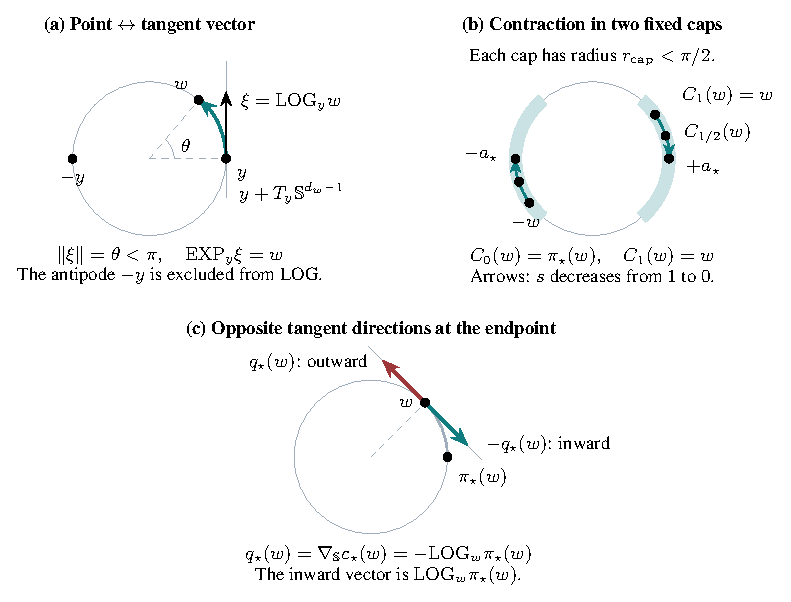
\includegraphics[width=\linewidth]{appendix_mf_dirac/spherical_geometry.pdf}
\caption{Spherical logarithms, exponentials, and pole contraction
(\cref{definition-spherical-logarithm-exponential,lem:fixed-assignment-contraction-geometry}).
(a) A point \(w\) at distance \(\theta<\pi\) from \(y\) corresponds to
the tangent vector \(\LOG_yw\) of length \(\theta\); \(\EXP_y\) maps it
back to \(w\). Vectors are drawn with their tails at their base points.
(b) Decreasing \(s\) from \(1\) to \(0\) in \(C_s(w)\) moves each point
to its assigned pole and preserves its cap.
(c) At the endpoint \(w\), \(q_\star(w)=\nabla_\Sphere c_\star(w)
=-\LOG_w\pi_\star(w)\) points outward; its negative points toward the
pole. The cost is \(c_\star(w)=d_\Sphere(w,\pi_\star(w))^2/2\).
Each circle is a great-circle cross section of the unit sphere; these
geometric paths do not represent a WGF trajectory.}
\label{fig:mf-spherical-geometry}
\end{figure}

\subsubsection{Tensorized objective}
We now rewrite the fitting loss as a sum of squared tensor residuals.

The sphere constraint gives a uniform bound on all moment tensors.
\begin{remark}
Under \cref{assumption:on-sphere}, the sphere constraint implies
\[
    \|T_{i,n}\|_{\mathrm{F}} \le 1,
    \qquad
    \|T_{i,n}^o\|_{\mathrm{F}} \le 1,
    \qquad i=1,2,
\]
for every $n\ge 0$. Under \cref{assumption:odd-symmetric-teacher},
the Hermite-moment expansions used below are finite sums.
\end{remark}

The next lemma is the algebraic bridge from the neural-network fitting loss to finite tensor residuals.

\begin{lemma}[Hermite expansion of the metric-regularized objective]
\label{lemma:EMN-expansion-F}
\textbf{Assumptions used.} \cref{assumption:on-sphere,assumption:odd-symmetric-teacher}.

Define
\begin{align}
    \mathcal M_p
    &\coloneq
    \sum_{\substack{n,m\ge 0\\ 0\le r\le \min(n,m)\\ p=n+m-2r}}
    c_{n,m,r}(a_n a_m^\top)\otimes \sym{T_{1,n}\contr{r} T_{2,m}},
    \\
    \mathcal M_p^o
    &\coloneq
    \sum_{\substack{n,m\ge 0\\ 0\le r\le \min(n,m)\\ p=n+m-2r}}
    c_{n,m,r}(a_n a_m^\top)\otimes \sym{T_{1,n}^o\contr{r} T_{2,m}^o},
    \\
    c_{n,m,r}
    \coloneq&
    r!\binom nr\binom mr
    \sqrt{\frac{(n+m-2r)!}{n!\,m!}},
    \qquad
    \Delta\mathcal M_p\coloneq \mathcal M_p-\mathcal M_p^o.
\end{align}
These residuals have both output-matrix indices and spatial tensor indices:
$\mathcal M_p,\mathcal M_p^o,\Delta\mathcal M_p
\in\mathbb R^{d_h\times d_h}\otimes\Sym^p(\mathbb R^{d_w})$.
For such a tensor $B$, write $B_{\alpha\beta}$ for its spatial tensor
at output indices $(\alpha,\beta)$. For $U\in\Sym^p(\mathbb R^{d_w})$
and $A\in\mathbb R^{d_h\times d_h}$, the two partial pairings mean
\begin{equation}
\label{eq:mf-matrix-tensor-partial-pairings}
\begin{aligned}
 \langle U,B\rangle_{\alpha\beta}
 &:=\langle U,B_{\alpha\beta}\rangle_{\rm HS},
 &\langle U,B\rangle&\in\mathbb R^{d_h\times d_h},\\
 \langle B,A\rangle_{\rm F}
 &:=\sum_{\alpha,\beta=1}^{d_h}A_{\alpha\beta}B_{\alpha\beta},
 &\langle B,A\rangle_{\rm F}&\in\Sym^p(\mathbb R^{d_w}),\\
 \|B\|_{\rm HS}^2
 &:=\sum_{\alpha,\beta=1}^{d_h}\|B_{\alpha\beta}\|_{\rm HS}^2.
\end{aligned}
\end{equation}
Thus pairing with $\Hertensor_p(z)$ contracts the spatial indices,
whereas pairing with $a_na_m^\top$ contracts the output indices.
Then
\begin{equation}
\label{eq:EMN-expanded-squared-chi2-objective}
    F(\mu)
    =
    \frac12\sum_{p\ge 0}\|\Delta\mathcal M_p\|_{\mathrm{HS}}^2
    +
    \frac{\lambdaReg}{p_W}Z_\pm(\mu_1,\mu_2)^{p_W/2}.
\end{equation}
The first term is the Hermite expansion of the fitting loss, and the second term is the antipodal Dirac metric regularizer from \eqref{eq:EMN-objective-squared-chi2}.
\end{lemma}

\begin{remark}
    Under \cref{assumption:odd-symmetric-teacher}, this tensor residual system becomes finite dimensional. The sums defining \(\mathcal M_p\) and \(\mathcal M_p^o\) reduce to indices \(n,m\in\mathcal O\).
\end{remark}
\begin{proof}
\noindent\textbf{Step 1: multiply the finite Hermite expansions.}
Throughout the proof, all
Hermite tensors are understood with the normalization used in
\cref{eq:normalized-hermite-tensor-orthogonality,eq:normalized-hermite-tensor-product-formula}, so that different homogeneous chaoses are
orthogonal in \(L^2\) under the law of \(z\).

For \(i=1,2\), the Hermite expansion of the feature map gives
\begin{equation}
    h_{\mu_i}(z)
    =
    \sum_{n\ge0}
    a_n\,
    \big\langle \Hertensor_n(z),T_{i,n}\big\rangle,
    \qquad
    T_{i,n}
    =
    \int_{\Sphere} w^{\otimes n}\,\dd\mu_i(w).
\end{equation}
Hence the matrix-valued product can be written as
\begin{align}
    h_{\mu_1}(z)h_{\mu_2}(z)^\top
    &=
    \sum_{n,m\ge0}
    a_n a_m^\top\,
    \big\langle \Hertensor_n(z),T_{1,n}\big\rangle
    \big\langle \Hertensor_m(z),T_{2,m}\big\rangle .
\end{align}
We now apply the Wiener-chaos product formula.  For symmetric tensors
\(A\in (\mathbb R^{d_w})^{\otimes n}\) and
\(B\in(\mathbb R^{d_w})^{\otimes m}\), one has
\begin{equation}
    \big\langle \Hertensor_n(z),A\big\rangle
    \big\langle \Hertensor_m(z),B\big\rangle
    =
    \sum_{r=0}^{\min(n,m)}
    c_{n,m,r}
    \Big\langle
        \Hertensor_{n+m-2r}(z),
        \sym{A\contr{r}B}
    \Big\rangle,
\end{equation}
where
\[
    c_{n,m,r}
    =
    r!\binom nr\binom mr \sqrt\frac{(n+m-2r)!}{n!m!}.
\]
Substituting \(A=T_{1,n}\) and \(B=T_{2,m}\), we obtain
\begin{align}
    h_{\mu_1}(z)h_{\mu_2}(z)^\top
    &=
    \sum_{n,m\ge0}
    \sum_{r=0}^{\min(n,m)}
    c_{n,m,r}
    (a_n a_m^\top)
    \Big\langle
        \Hertensor_{n+m-2r}(z),
        \sym{T_{1,n}\contr{r}T_{2,m}}
    \Big\rangle .
\end{align}
Collecting all terms with the same Hermite degree $p=n+m-2r,$
we can rewrite this as
\begin{equation}
    h_{\mu_1}(z)h_{\mu_2}(z)^\top
    =
    \sum_{p\ge0}
    \big\langle \Hertensor_p(z),\mathcal M_p\big\rangle,
\end{equation}
where the coefficient tensor is precisely
\begin{equation}
    \mathcal M_p
    =
    \sum_{\substack{n,m\ge0\\0\le r\le \min(n,m)\\p=n+m-2r}}
    c_{n,m,r}
    (a_na_m^\top)\otimes
    \sym{T_{1,n}\contr{r}T_{2,m}}.
\end{equation}
The same calculation applied to the teacher measures gives
\begin{equation}
    h_{\mu_1^o}(z)h_{\mu_2^o}(z)^\top
    =
    \sum_{p\ge0}
    \big\langle \Hertensor_p(z),\mathcal M_p^o\big\rangle,
\end{equation}
with
\begin{equation}
    \mathcal M_p^o
    =
    \sum_{\substack{n,m\ge0\\0\le r\le \min(n,m)\\p=n+m-2r}}
    c_{n,m,r}
    (a_na_m^\top)\otimes
    \sym{T_{1,n}^o\contr{r}T_{2,m}^o}.
\end{equation}
Therefore
\begin{equation}
    h_{\mu_1}(z)h_{\mu_2}(z)^\top
    -
    h_{\mu_1^o}(z)h_{\mu_2^o}(z)^\top
    =
    \sum_{p\ge0}
    \big\langle \Hertensor_p(z),\Delta\mathcal M_p\big\rangle,
    \qquad
    \Delta\mathcal M_p=\mathcal M_p-\mathcal M_p^o .
\end{equation}

\par\noindent\textbf{Step 2: use orthogonality to sum the residual squares.}
We now take the \(L^2\)-norm in \(z\), with Frobenius norm in the
matrix output.  Since distinct Hermite chaoses are orthogonal, all
cross terms with \(p\neq q\) vanish:
\begin{align}
    &\E_z
    \Big[
        \big\|
        h_{\mu_1}(z)h_{\mu_2}(z)^\top
        -
        h_{\mu_1^o}(z)h_{\mu_2^o}(z)^\top
        \big\|_{\mathrm F}^2
    \Big]
    \notag\\
    &\qquad =
    \sum_{p,q\ge0}
    \E_z
    \Big[
        \Big\langle
            \big\langle \Hertensor_p(z),\Delta\mathcal M_p\big\rangle,
            \big\langle \Hertensor_q(z),\Delta\mathcal M_q\big\rangle
        \Big\rangle_{\mathrm F}
    \Big]
    \notag\\
    &\qquad =
    \sum_{p\ge0}
    \|\Delta\mathcal M_p\|_{\mathrm{HS}}^2 .
\end{align}
Consequently,
\begin{equation}
    \frac12
    \E_z
    \Big[
        \big\|
        h_{\mu_1^o}(z)h_{\mu_2^o}(z)^\top
        -
        h_{\mu_1}(z)h_{\mu_2}(z)^\top
        \big\|_{\mathrm F}^2
    \Big]
    =
    \frac12
    \sum_{p\ge0}
    \|\Delta\mathcal M_p\|_{\mathrm{HS}}^2 .
\end{equation}

It remains only to identify the regularization term.  By definition of
\(Z_\pm\), the metric regularization term in \eqref{eq:EMN-objective-squared-chi2} is exactly
\[
    \frac{\lambdaReg}{p_W}Z_\pm(\mu_1,\mu_2)^{p_W/2}.
\]
This proves \eqref{eq:EMN-expanded-squared-chi2-objective}.
\end{proof}

\paragraph{Bridge to the geometry overview.}
This tensorized form is the coordinate system used in the curvature arguments below.
Thus the model is reduced to a tensor residual system: the fitting loss is the squared Hilbert-Schmidt norm of the residuals \(\Delta\mathcal M_p\), while the metric term controls distance to the antipodal pair. In the next subsection, the active odd moments are recombined into symmetric and anti-symmetric coordinates to describe the curvature transition.
